\chapter{PRIMEIRA ITERAÇÃO}
\label{cap3}

A primeira iteração do algoritmo de inversão tem por objetivo a obtenção do gradiente de
velocidades em profundidade do modelo de velocidades de background, este resultado é oque
chamamos de primeira iteração. O modelo inicial utilizado é um modelo de velocidades homogêneo
e de velocidade constante igual a 1.5Km/s correspondente a velocidade próxima da superfície de aquisição. 

\begin{figure}[H]
\caption{Picking dos tempos de trânsito sobre um refletor da seção empilhada ERC. Os pontos
em amarelo são os pares $t_0$ e $m_0$ escolhidos.}
\begin{center}
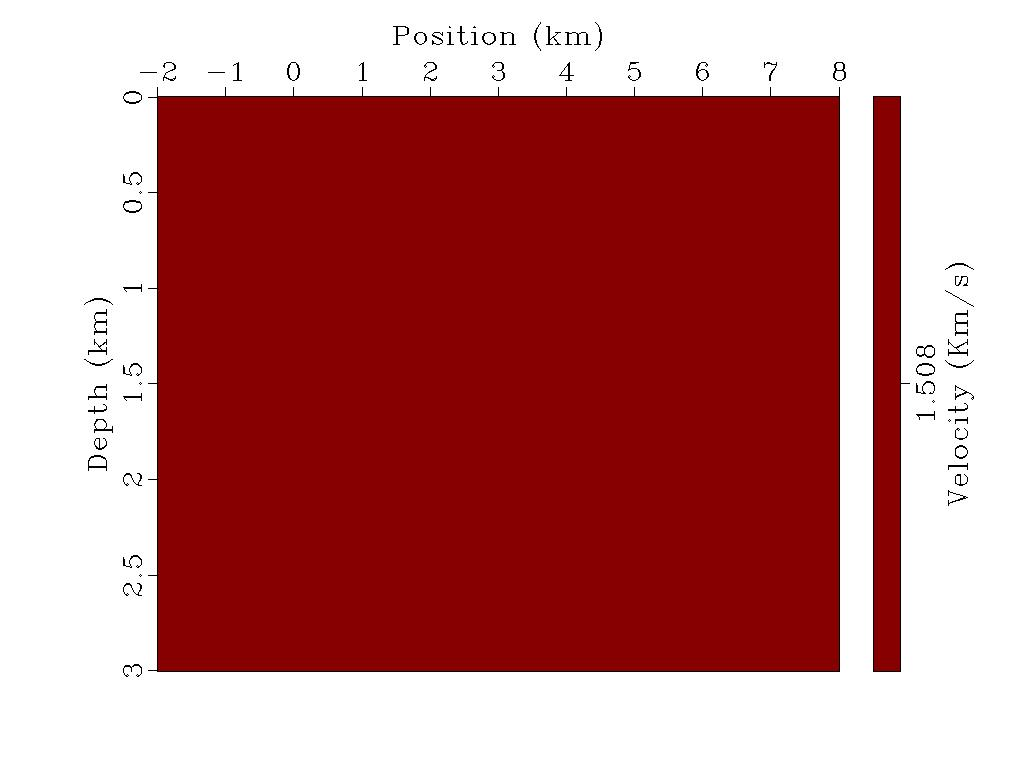
\includegraphics[scale=0.3]{images/ctevel.jpeg}
\vspace{-0.3cm}
\end{center}
\begin{center}
 Fonte: Do Autor.
\end{center}
\label{fig:3.1}
\end{figure}


Nesta etapa, é utilizado o algoritmo Very Fast Simulated Annealing (VFSA) para realizar a otimização do
gradiente de profundidade do modelo de velocidades. O modelo de velocidades é atualizado a cada iteração do
algoritmo para cada valor do gradiente e segue a seguinte função de velocidades:

\begin{equation}
\label{eq:3.1}
v(z)=z g_z+v_0
\end{equation}

Em \ref{eq:3.1} a velocidade $v(z)$ cresce linearmente com a profundidade.

\begin{figure}[H]
\caption{Picking dos tempos de trânsito sobre um refletor da seção empilhada ERC. Os pontos
em amarelo são os pares $t_0$ e $m_0$ escolhidos.}
\begin{center}
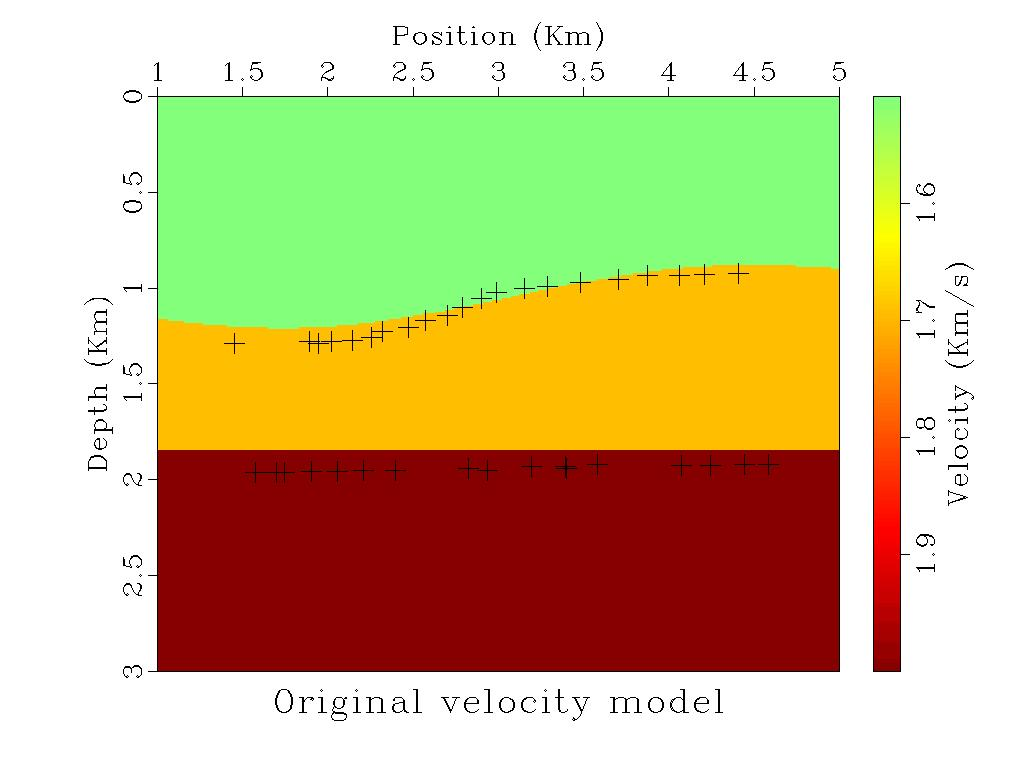
\includegraphics[scale=0.3]{images/gzvel.jpeg}
\vspace{-0.3cm}
\end{center}
\begin{center}
 Fonte: Do Autor.
\end{center}
\label{fig:3.2}
\end{figure}


O critério de otimização do gradiente de velocidades é 
TODO: critério de otimização semblance, tempos de trânsito e CRE

Nesta etapa, é utilizado o algoritmo Very Fast Simulated Annealing (VFSA) para realizar a otimização do
gradiente de profundidade do modelo de velocidades. O modelo de velocidades é atualizado a cada iteração do
algoritmo para cada valor do gradiente e segue a seguinte função de velocidades:

\begin{equation}
\label{eq:4.1}
v(z)=z g_z+v_0
\end{equation}

Em \ref{eq:4.1} a velocidade $v(z)$ cresce linearmente com a profundidade.

FOTO MODELO GZ

O critério de otimização do gradiente de velocidades é 
TODO: critério de otimização semblance, tempos de trânsito e CRE



